\documentclass[11pt]{article}

\usepackage{color}
\usepackage[usenames,dvipsnames,svgnames,table]{xcolor}

\usepackage{graphicx}
\usepackage{amsmath}
\usepackage{amssymb}
\usepackage{eulervm}
\usepackage{charter}
\usepackage{exercise}
\PassOptionsToPackage{hyphens}{url}\usepackage{hyperref}
\hypersetup{colorlinks=true,linkcolor=DarkRed,urlcolor=DarkRed}
\usepackage{float}
\usepackage{enumitem}
\usepackage{bm}

\newcommand{\p}{\;\text{.}}

\newcommand{\R}{{\mathbb R}}
\newcommand{\N}{{\mathbb N}}
\newcommand{\E}{{\mathbb E}}

\newcommand{\U}{{\bm U}}
\newcommand{\V}{{\bm V}}
\newcommand{\W}{{\bm W}}
\newcommand{\A}{{\bm A}}
\newcommand{\B}{{\bm B}}
\newcommand{\C}{{\bm C}}
\newcommand{\ba}{{\bm a}}
\newcommand{\bb}{{\bm b}}
\newcommand{\boc}{{\bm c}}
\newcommand{\bu}{{\bm u}}
\newcommand{\bv}{{\bm v}}
\newcommand{\bw}{{\bm w}}
\newcommand{\x}{{\bm x}}
\newcommand{\y}{{\bm y}}
\newcommand{\z}{{\bm z}}
\newcommand{\X}{{\bm X}}
\newcommand{\Y}{{\bm Y}}
\newcommand{\Z}{{\bm Z}}
\newcommand{\bt}{{\bm t}}
\newcommand{\ma}[1]{\begin{pmatrix}#1\end{pmatrix}}

\DeclareMathOperator*{\argmin}{arg\,min}
\DeclareMathOperator*{\argmax}{arg\,max}

\newcommand{\ans}[2]{{\leavevmode\color{OliveGreen}#2}} % no answers
% \newcommand{\ans}[2]{{\leavevmode\color{OliveGreen}#1}} % answers

\newcommand{\red}[1]{{\textcolor{Red}{#1}}}
\definecolor{myred}{HTML}{C82506}
\definecolor{myblue}{HTML}{0365C0}
\definecolor{mygreen}{HTML}{00882B}
\definecolor{myorange}{HTML}{DE6A10}
\definecolor{mypurple}{HTML}{773F9B}
\definecolor{myyellow}{HTML}{DCBD23}

\newcommand{\rc}[1]{{\textcolor{myred}{ #1 }}}
\newcommand{\gc}[1]{{\textcolor{mygreen}{ #1 }}}
\newcommand{\bc}[1]{{\textcolor{myblue}{ #1 }}}
\newcommand{\kc}[1]{{\textcolor{Gray}{ #1 }}}
\newcommand{\oc}[1]{{\textcolor{myorange}{ #1 }}}
\newcommand{\pc}[1]{{\textcolor{mypurple}{ #1 }}}
\newcommand{\yc}[1]{{\textcolor{myyellow}{ #1 }}}

\newcommand{\kp}{{\kc{\partial}}}
% Exam questions
\newcommand{\trueorfalse}{\linebreak \textbf{A } True ~~ \textbf{B } False}
\newcommand{\choices}[4]{\linebreak\noindent\textbf{A } #1~~\textbf{B } #2~~\textbf{C } #3~~\textbf{D } #4}
%\newcommand{\choicesnum}[4]{\linebreak\noindent{\fill}\textbf{A } \np{#1}~~\textbf{B } \np{#2}~~\textbf{C } \np{#3}~~\textbf{D } \np{#4}}
%\newcommand{\twochoices}[2]{\linebreak\noindent\textbf{A } #1~~\textbf{B } #2}
%\newcommand{\threechoices}[3]{\linebreak\noinden\textbf{A } #1~~\textbf{B } #2~~\textbf{C } #3}
\newcommand{\choicesv}[4]{\\ \begin{minipage}{\textwidth}\vspace{4pt}\noindent\textbf{A } #1\\ \noindent\textbf{B } #2\\ \noindent\textbf{C } #3\\ \noindent\textbf{D } #4\end{minipage}}

% Homework questions
\newcommand{\qu}[0]{%
  \addtocounter{Question}{1}%
  \noindent \textbf{question \theQuestion:}
}


\newcommand{\an}{\ans{\checkmark}{}}

\title{Week 1: Preliminaries}
\author{\url{http://mlvu.github.io}}

\usepackage{tikz}

\newcommand\tikzmark[1]{%
  \tikz[overlay,remember picture,baseline] \node [anchor=base] (#1) {};}

\newcommand\MyLine[3][]{%
  \begin{tikzpicture}[overlay,remember picture]
    \draw[#1] (#2.north west) -- (#3.south east);
  \end{tikzpicture}}

\begin{document}

\maketitle

\noindent This week, the homework will be a review of subjects you should be familiar with already. Machine learning is built mostly on three types of math: \emph{Linear Algebra}, \emph{Calculus} and \emph{Probability Theory}. Luckily, we only use a very limited number of concepts from each, so even if you don't know these subjects or don't know them well, it shouldn't take too much work to get up to speed.

Here we'll review some linear algebra and some calculus, saving the probability for later. We'll also review three concepts that you should become very familiar with to follow machine learning theory: sums, expectations and logarithms. Even if you know these in principle, you should take the time to get comfortable with them.

This homework should give you an indication of whether you have a sufficient grasp of the preliminaries. If you struggle with anything, please follow the links provided to brush up, before continuing with next week's homework. 

\section{Sums, expectations and logarithms}

You've probably encountered all three of these before. However, in the lectures, we will often see long derivations which require you to to be very familiar with these in order to follow all the steps. If you find yourself baffled by some of the math in the lecture, you can probably get a lot closer by just practising your sums, expectations and logarithms a little.

\paragraph{Sums} Sigma ($\Sigma$) notation is simply a concise way of writing down long sums. Assume we have a list of numbers $a_\rc{1}, a_\rc{2}, a_\rc{3}, a_\rc{4}, a_\rc{5}$. We can write:
\[
a_\rc{1} + a_\rc{2} + a_\rc{3} + a_\rc{4} + a_\rc{5}
\]
but we can also write
\[
\sum_{\rc{i}=1}^5 a_\rc{i} \;\;\;\;\text{or}\;\;\;\;\textstyle\sum_{\rc{i}=1}^5 a_\rc{i} 
\]
The bit below the sigma tells you which symbol is used as an index ($\rc{i}$) to iterate over the elements to sum over, and what the first value is ($1$). The bit above the sigma tells you what the last value of the index is. \footnotemark

\footnotetext{If you're an experienced programmer, it may be helpful to think of this as a \texttt{for} loop: something like $\texttt{for(int \rc{i} = 1; \rc{i} < 6; \rc{i}++)}\ldots$.}

Since this is a very dense notation, it's often simplified by leaving out the start and end values, assuming that they can be figured out from context:
\[
\sum_\rc{i} a_\rc{i}
\]
Sums can be nested as well (using a sum within a sum). This is not a special notation, it simply follows from the definition. You  can `unpack' these by turning the sigmas into a regular sum one by one:
\begin{align*}
&\sum_{\rc{i}=1}^{2} \sum_{\bc{j}=1}^{3} a_\rc{i} b_\bc{j} \\ 
 &= \sum_{\bc{j}=1}^{3} a_\rc{1} b_\bc{j} + \sum_{\bc{j}=1}^{3} a_\rc{2} b_\bc{j} \\
 &= (a_\rc{1} b_\bc{1} + a_\rc{1}b_\bc{2} + a_\rc{1}b_\bc{3}) + (a_\rc{2}b_\bc{1} + a_\rc{2}b_\bc{2} + a_\rc{2}b_\bc{3}) \\
\end{align*}
For nested sums, the indices are often combined into a single sigma:
\[
\sum_{\rc{i}, \bc{j}} a_\rc{i} b_\bc{j}= \sum_\rc{i} \sum_\bc{j} a_\rc{i} b_\bc{j} 
\]


\qu \noindent Let $x_\rc{1} = 5, x_\rc{2} = 1, x_\rc{3} = 4, x_\rc{4} = 1, x_\rc{5} = 3$. Compute the following values:
\begin{enumerate}
	\item $\sum_\rc{i} x_\rc{i}$ \ans{$= 5 + 1 + 4 + 1 + 3 = 14$}{}
	\item $\sum_\rc{i} 2 \cdot x_\rc{i}$ \ans{$= 10 + 2 + 8 + 2 + 6 = 28$}{}
	\item $2 \cdot \sum_\rc{i} x_\rc{i}$ \ans{$= 2 \cdot (5 + 1+ 4 + 1 + 3) = 28$}{}
	\item $\sum_{\rc{i}=1}^{3} x_\rc{i}$ \ans{$= (5 + 1 + 4) = 10 $}{}
	\item $\sum_{\rc{i}=1}^{x_5} x_\rc{i}$ \ans{$= (5 + 1 + 4) = 10$. Note that the answer is \emph{not} 14. We sum until the \emph{\rc{index}} is equal to $x_5$ (which is equal to 3), not until we enounter $x_5$.}{}
	\item $\sum_{\rc{i}=1}^{3} \rc{i} \cdot x_\rc{i}$ \ans{$= (1 \cdot 5 + 2 \cdot 1+ 3\cdot 4) = 19 $}{}
\end{enumerate}

\qu Which of the following are always true? If you struggle, try rewriting  as a normal sum, and using what you already know about sums. The variable $\kc{c}$ is a constant.
\begin{enumerate}
\item $\sum_\rc{i} \kc{c}y_\rc{i} = \kc{c}\sum_\rc{i} y_\rc{i}$ \ans{True. This is the equivalent of ``moving a constant outside brackets.'' For instance $cx + cy + cz = c(x+ y + z)$}{}
\item $\sum_\rc{i} (\kc{c} + y_\rc{i}) = \kc{c} + \sum_\rc{i} y_\rc{i}$ \ans{False. On the left $\kc{c}$ is added to every term, and on the right it is added only once.}{}
\item $\sum_{\rc{i}=1}^\yc{n} (\kc{c} + y_\rc{i}) = \yc{n}\kc{c} + \sum_{\rc{i}=1}^\yc{n} y_\rc{i}$ \ans{True. On the left we add $c$ $n$ times, which is the same as adding $nc$ once.}{}
\item $\sum_\rc{i} (x_\rc{i} + y_\rc{i}) = \left(\sum_\rc{i} x_\rc{i}\right) + \left(\sum_\rc{i} y_\rc{i}\right)$ \ans{True. Think of this as re-arranging the terms of the sum: $(x_1 + y_1 + x_2 + y_2 + x_3 + y_3) = (x_1 + x_2 + x_3) + (y_1 + y_2 + y_3)$}{}
\item $\sum_\rc{i} \sum_\bc{j} a_\rc{i} b_\bc{j} = \sum_\bc{j} \sum_\rc{i} a_\rc{i}b_\bc{j}$ \ans{True. Looping over all $a$ and summing each with every $b$  is the same as looping over all $b$ and summing each with every $a$.}{}
\item $\sum_\rc{i} a_\rc{i}b_\rc{i} = \left(\sum_\rc{i} a_\rc{i} \right) \left( \sum_\rc{i} b_\rc{i}\right)$ \ans{False. $1\cdot 4 + 3 \cdot 2 \neq (1+3)(4+2)$}{}

\end{enumerate}

\noindent It can be a little ambiguous where the sum operator ends. For instance, in $\sum_\rc{i} x_\rc{i} + \kc{c}$, we don't know whether the $\kc{c}$ should be added once, or for every term in the sum.  There's no official standard, and authors should make sure to write sums in an unambiguous way. For instance $\sum_\rc{i} \kc{c} + x_\rc{i}$ or $\kc{c} + \sum_\rc{i} x_\rc{i}$ or simply $\sum_\rc{i} (\kc{c} + x_\rc{i})$.

The capital pi $\Pi$ works in exactly the same way as the $\Sigma$ operator, but describes a \emph{product}:
\[
\prod_{\rc{i}=1}^4 \rc{i} = 24
\]

More practice? Try these links:
\begin{itemize}
\item \url{https://www.khanacademy.org/math/algebra2/sequences-and-series/alg2-sigma-notation/e/evaluating-basic-sigma-notation}
\item \url{https://www.mathsisfun.com/algebra/sigma-notation.html}
\item \url{https://www.youtube.com/watch?v=TjMLzklnn2c}	
\end{itemize}


\paragraph{Expectations} An expectation is nothing more than a sum, with each term weighted by a probability. Let's say you are playing a game where you roll a die, and you receive the number of  eyes rolled in euros. Your expected reward is:
\[
\frac{1}{6} \cdot 1 + \frac{1}{6} \cdot 2 + \frac{1}{6} \cdot 3 + \frac{1}{6} \cdot 4 + \frac{1}{6} \cdot 5 + \frac{1}{6} \cdot 6 = \frac{21}{6} = 3.5
\]
In general, if you have a random variable $\bc{V}$ (an experiment with a numeric outcome) which has possible outcomes $\rc{1}, \rc{2}, \ldots$ with associated values $v_\rc{1}, v_\rc{2}, \ldots$ and associated probabilities $p_\rc{1}, p_\rc{2}, \ldots$, the \textbf{expected value} of the experiment is written as
\begin{equation}
\ex (\bc{V}) = \sum_\rc{i} p_\rc{i} v_\rc{i} \label{line:exp}
\end{equation}
The brackets can be omitted at the author's discretion. If multiple probability distributions are applicable, the choice of distribution may be indicated in the subscript $\ex_p \bc{V}$.

We can also extend the experiment by applying a function to the outcome, and computing the expected value over the result. Say that $\bc{V}$ describes a betting game with winnings $v_\rc{i}$, but you will have to pay a 20\% tax over whatever you win. Then, the expectation for the amount of money you actually get to keep is 

\[
\ex (\kc{0.8} \cdot \bc{V})= \sum_\rc{i} p_\rc{i} \cdot \kc{0.8} \cdot v_\rc{i} 
\]

\qu Because the expectation is basically a sum, most of the things that hold for sums, also hold for expectations.
Show that the following hold by applying what you know about sums. If you get stuck, try expanding the expectation into a sum, as in (\ref{line:exp}).

\begin{enumerate}
	\item $\ex (\kc{c}\cdot \bc{V}) = \kc{c} \cdot \ex(\bc{V})$ (homogeneity) \ans{
\begin{align*}
	\ex_\bc{V} (\kc{c}\cdot \bc{V})
	= \sum_\rc{i} p_\rc{i} \kc{c} v_\rc{i} 
	= \kc{c} \sum_\rc{i} p_\rc{i} v_\rc{i}
 	= \kc{c} \cdot \ex_\bc{V}(\bc{V})
\end{align*}
}{} 
\item Let $\bc{V}$ and $\rc{W}$ have different numeric values, $\bc{v}_i$ and $\rc{w}_i$, for outcomes with the same probability $p_i$. Then $\ex(\bc{V}) + \ex(\rc{W}) = \ex(\bc{V} + \rc{W})$ (additivity) \label{line:sum} \ans{
\begin{align*}
	\ex&(\bc{V}) + \ex(\rc{W}) \\
	&= \sum_i p_i \bc{v_i}  + \sum_i p_i \rc{w_i} \\
	&= \sum_i p_i \bc{v_i}  + p_i \rc{w_i} = \sum_i p_i (\bc{v_i}  + \rc{w_i})\\
	&= \ex(\bc{V} + \rc{W})
\end{align*}
}{} 
\item $\ex(\bc{V}) + \ex(\sin(\bc{V})) = \ex(\bc{V} + \sin(\bc{V}))$ \label{line:sum} \ans{This follows directly from additivity (just set $\rc{W} = \sin{\bc{V}}$)}{} 
\item $\ex\left((\bc{V} - \ex\bc{V})^2\right) = \ex(\bc{V}^2) - (\ex\bc{V})^2 $ \label{line:variance} \ans{
\begin{align*}
	\ex&\left((\bc{V} - \ex\bc{V})^2\right) &  \\ 
	&=\ex\left(\bc{V}^2 - 2\bc{V}\ex\bc{V} + (\ex\bc{V})^2)\right) &\kc{\text{expand:} (a+b)^2 = a^2 + 2ab + b^2} \\
	&=\ex(\bc{V}^2) - 2\ex(\bc{V})\ex(\bc{V}) + \ex(\ex\bc{V})^2& \kc{\text{use additivity \& homogeneity}} \\	
	&=\ex(\bc{V}^2) - 2(\ex\bc{V})^2 + (\ex\bc{V})^2 &\kc{\text{$\ex(\ex \bc{V})^2$ is an $\ex$ over a constant.}}  \\	
	&= \ex(\bc{V}^2) - (\ex\bc{V})^2 &
\end{align*}
}{}

\end{enumerate}

\noindent If your outcomes form a \emph{continuum}, like real-valued numbers (e.g. if you sample from a normal distribution), the expectation is defined with an integral instead of a sum ($\ex_\bc{V} = \int_\rc{x} p(\rc{x})\bc{v}(\rc{x}) \kc{dx}$). Since the integral has most of the same properties as the sum, you can use both types of expectation in the same way. \footnote{In fact, we use this trick in the course to hide some of the complexity: by talking about expectations without unpacking the notations, we can discuss many aspects of distributions on continuous spaces, without ever using integrals.}

More practice? Try these links:
\begin{itemize}
\item \url{https://www.khanacademy.org/math/probability/probability-geometry/expected-value-geo/a/expected-value-basic}	
\end{itemize}

\paragraph{Logarithms} The \emph{logarithm} is nothing more than the inverse of the exponential. If $\rc{y} = b^\bc{x}$ then $\bc{x} = \log_b \rc{y}$. 

Since $100 = 10\cdot 10 = 10^2$, $1000 = 10 \cdot10\cdot 10^3$ and so on, $log_{10} x$ gives us an indication of the \emph{order of magnitude} of $x$. That is, how many digits do we need to write down $x$. 

For instance $log_{10} (314) \approx 2.5$ and  $log_{10} (31400) \approx 4.5$. In other words, if two numbers have the same order or magnitude, the difference between their base-10 logarithms will be at most 1. 

This also works for numbers smaller than one, except that the logarithm becomes negative: $log_{10} (0.1) = -1$, $log_{10} (0.01) = -2$, $log_{10} (0.001) = -3$ and so on. 

The base-10 logarithm is between 1 and 2 for all numbers between  0 and 10, between 2 and 3 for all numbers between 10 and 100, between 3 and 4 for all numbers between 100 and 1000 and so on.

For bases other than 10, it's not quite so neat, but the same principle holds: \textbf{all numbers with a given order of magnitude are squeezed into a constant-sized interval}. 

There are two main reasons why it's such a useful function in machine learning:
\begin{itemize}
\item The standard numerical representations used in computers have \emph{limited precision}: they cannot accurately represent differences smaller than about $10^{-16}$. Instead of storing the actual number, \emph{we can store the logarithm of the number}. This is useful, for instance, in representing probabilities. Since our probabilities are usually guesses anyway, we don't care as much about the difference between 0.0004 and 0.00035 as we do about the difference between $10^{-21}$ and $10^{-24}$. If we store the logarithm of the probability, the second difference remains clear, even if the actual probability is far too small to store.
\item Taking the logarithm \textbf{turns a product into a sum}: \begin{align*}\log (\rc{a}\cdot\bc{b}\cdot\gc{c}) &= \log \rc{a} + \log \bc{b} + \log \gc{c} \\ \textstyle \log \prod_\rc{i} x_\rc{i} &= \textstyle \sum_\rc{i}\log x_\rc{i}
 \end{align*} Sums are much easier to analyze and manipulate. This can be a tremendous help in working out derivatives and in other symbolic manipulation.
\end{itemize}



\qu Which of the following are true for all $\bc{a}, \oc{b}$? If true show why, from the following facts:
\begin{itemize}
\item If $x = c^y$ then $y = \log_c x$ (and vice versa).
\item $c^x \cdot c^y = c^{x + y}$ (check that you have an intuition for why this is true).
\end{itemize}
\noindent If not true, give a counterexample. 

\begin{enumerate}
\item $\log_\oc{b} \left(\oc{b}^\bc{a}\right) = \bc{a}$ \label{line:cancel}\ans{True. Note that (by definition) if $x = \log_b(y)$, then $y = b^x$. Therefore if $\log_\oc{b} \left(\oc{b}^\bc{a}\right) = x$, then $\oc{b}^x = \oc{b}^\bc{a}$, so $x=\bc{a}$. For some intuition, note that we are applying a function to \bc{$a$} and then applying the inverse to the result, so it should not be surprising that we end up with $\bc{a}$ again.  Note also the special case $\log_\oc{b} \left(\oc{b}\right) = \log_\oc{b} \left(\oc{b}^\bc{1}\right) = \bc{1}$.}{}
\item $\oc{b}^{\log_\oc{b} \bc{a}} = \bc{a}$\label{line:cancel2} \ans{True. As before, we are applying a function and then its inverse. If $x = b^y$ then $y = \log_b x$. Therefore if $x = \oc{b}^{\log_\oc{b}\bc{a}}$, then $\log_\oc{b} x = \log_\oc{b} \bc{a}$, so $x = \bc{a}$}{}
\item $\log_c \bc{a} + \log_c \oc{b} = \log_c (\bc{a}\oc{b})$\label{line:prod}. Hint: let $\bc{a'} = \log_c{\bc{a}}$ and $\oc{b'} = \log_c{\oc{b}}$ and apply one of the rules given. \ans{
\begin{align*}
c^{\bc{a'}} \cdot c^{\oc{b'}} &= c^{\bc{a'} + \oc{b'}} & \\
c^{\log_c{\bc{a}}} \cdot c^{\log_c{\oc{b}}} &= c^{\log_c{\bc{a}} + \log_c{\oc{b}}} & \\
\bc{a} \cdot \oc{b} &= c^{\log_c{\bc{a}} + \log_c{\oc{b}}} & \text{apply (\ref{line:cancel2})} \\
\log_c\left( \bc{a}\oc{b}\right) &= \log_c{c^{\log_c{\bc{a}} + \log_c{\oc{b}}}} &\text{take $\log_c$ on both sides} \\
\log_c\left( \bc{a}\oc{b}\right) &= \log_c{\bc{a}} + \log_c{\oc{b}} &\text{apply (\ref{line:cancel}) in the righthand side} \\
\end{align*}
}{}

\item $\log (\bc{a}^\oc{b}) = \oc{b} \log (\bc{a})$ \ans{True. Note that $\bc{a}^\oc{b}$ is just a multiplication $\bc{a} \cdot \bc{a} \cdot \ldots$, with $\oc{b}$ factors. Applying (\ref{line:prod}), we can turn this into a \emph{sum} with $\oc{b}$ \emph{terms}: $\log(\bc{a}^\oc{b}) = \log(\prod_{i=1}^\oc{b}\bc{a}) = \sum_{i=1}^\oc{b} \log \bc{a} = \oc{b} \log\bc{a}$}{}
\item $\log (\bc{a} + \oc{b}) = \log(\oc{b}) \cdot \log(\bc{a})$ \ans{False. If you see a sum inside a logarithm there's (sadly) no straightforward way to take it outside the log. Counterexample $\log_{10}(10 + 10) \neq \log_{10}(10) \cdot \log_{10}(10) $}{}
\item $\log (\bc{a}/\oc{b}) = \log (\bc{a}) - \log{(\oc{b})}$ \ans{True. \\$\log (\bc{a}/\oc{b}) = \log (\bc{a} \frac{1}{\oc{b}}) = \log (\bc{a} \oc{b}^{-1}) = \log \bc{a} +  \log (\oc{b}^{-1})= \log \bc{a} + (-1) \log (\oc{b})$}{}
\end{enumerate}

More practice? Try these links:
\begin{itemize}
\item \url{http://www.oxfordmathcenter.com/drupal7/node/532}
\item \url{https://www.khanacademy.org/math/algebra2/exponential-and-logarithmic-functions}
\item \url{https://study.com/academy/lesson/exponentials-and-logarithms-graphing-and-property-review.html}
\end{itemize}

\section{Linear Algebra}

A \textbf{vector} is a list of numbers, of a fixed length. The length (how many numbers there are in the vector) is its \emph{dimension}. Here is a vector of dimension 4:
\[
\x = \begin{pmatrix}3 \\ 3.1 \\- 2.5 \\0.1\end{pmatrix}
\] 

\noindent In our course materials, the variable name for a vector is a \textbf{bold} lowercase letter. To indicate the individual elements of the vector, we use the non-bold version of the letter, subscripted with an index: $x_3 = -2.5$. The notation $\x \in \R^4$ means that $\x$ is a vector consisting of four, real-valued numbers.

Vectors are often used to denote points or directions in space. For instance, for a vector in $\R^2$:

\begin{figure}[H]
\centering
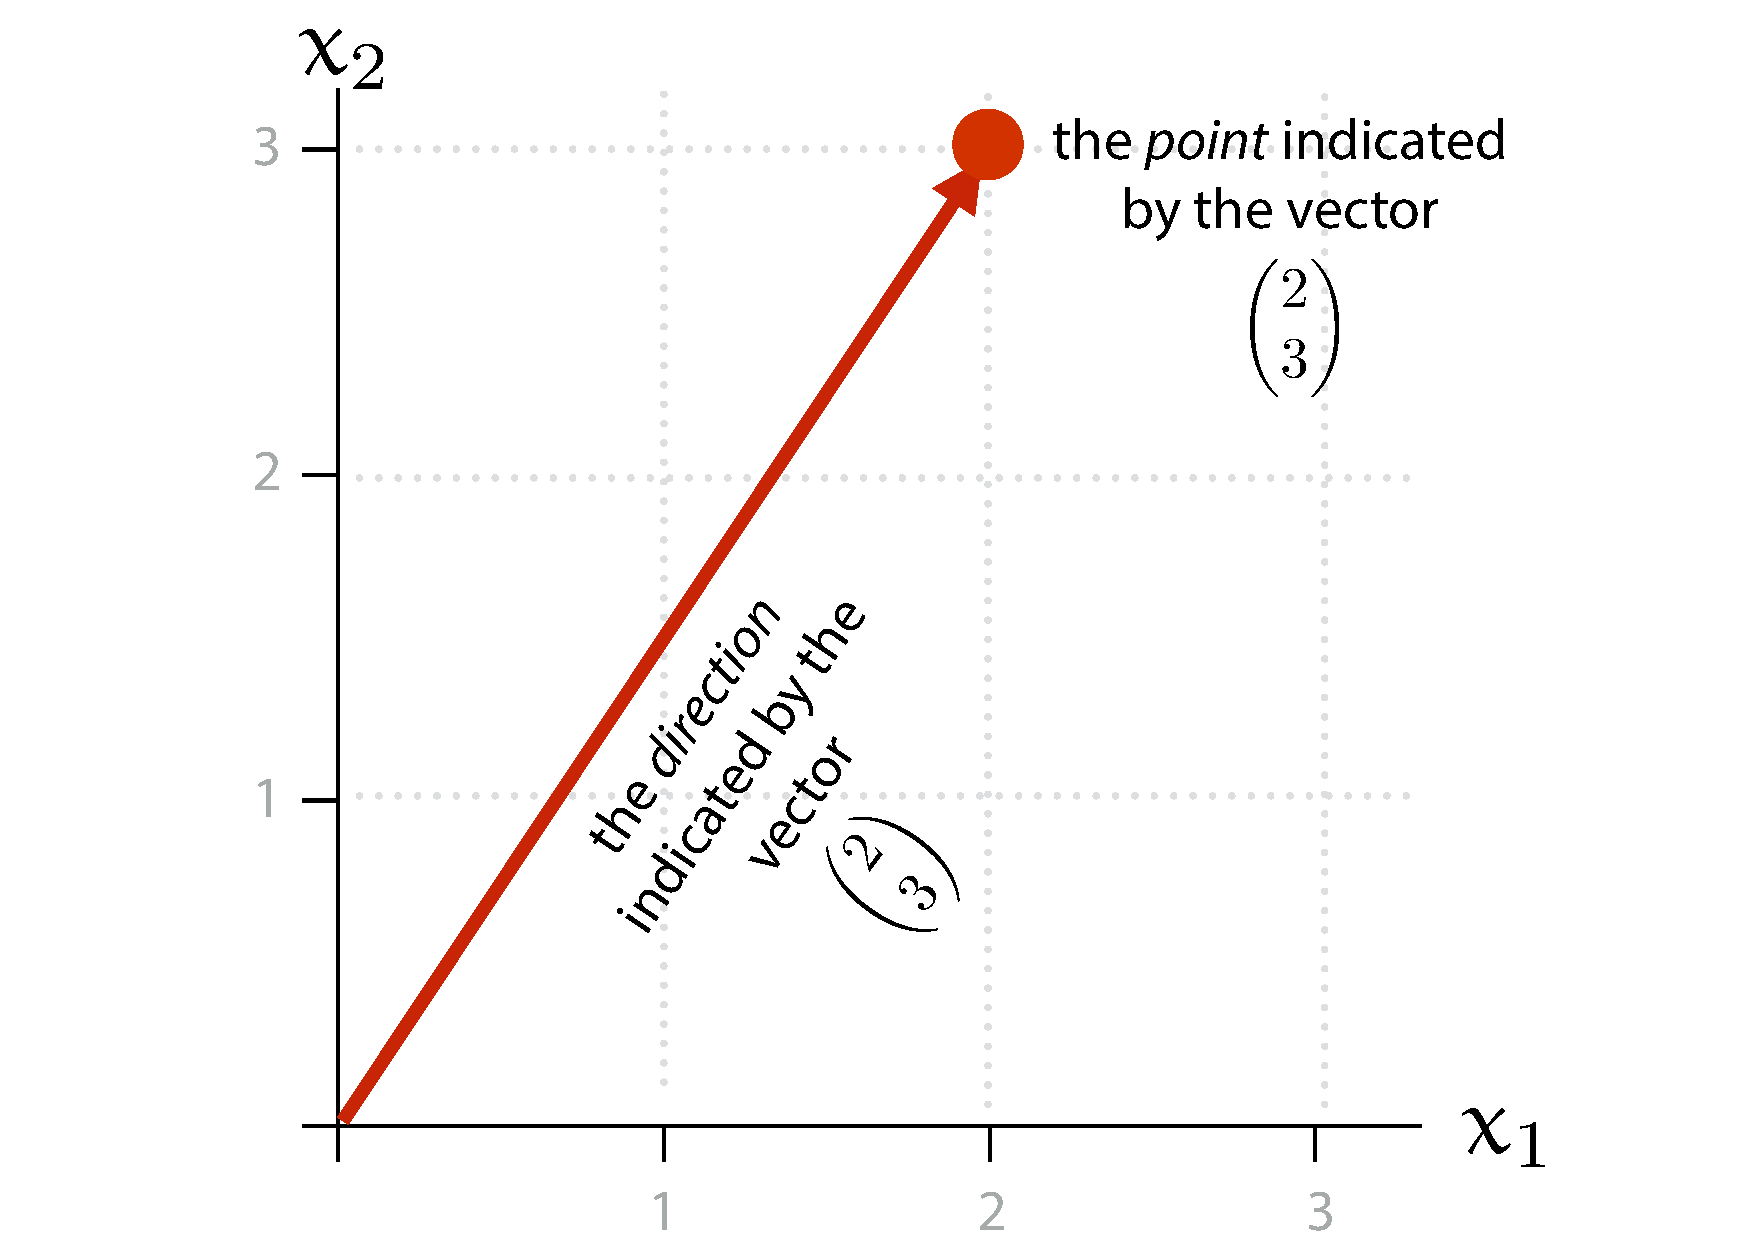
\includegraphics[width=0.7\linewidth]{vector}
\caption{Vectors as points and vectors as directions.}
\label{figure:vector}
\end{figure}

\noindent If we think of the vector $\x$ as an arrow (as shown in Figure~\ref{figure:vector}), the length of that arrow, denoted $||\x||$, is \footnotemark
\[
||\x|| = \sqrt{\textstyle\sum_\rc{i} {x_\rc{i}}^2}\p
\]

\footnotetext{This follows from the Pythagorean theorem. For a 2D example, see Figure~\ref{figure:vector}. Let $l = ||\x||$. By Pythagoras $l^2 = {x_1}^2 + {x_2}^2$, so $l = \sqrt{{x_1}^2 + {x_2}^2}$.}

\noindent A \textbf{matrix} is also a bunch of numbers, but arranged in a \emph{grid}. Here is an example of a $3 \times 4$ matrix:
\[
\W = \begin{pmatrix}3 & 5 & 1.1 & 0 \\ 0 & 3.1 & 3  & 1\\ 1 & 9 & - 2.5 & 0\end{pmatrix}
\] 

\noindent In our course materials, the variable name for a matrix is a \textbf{bold} \emph{upper}case letter. To indicate the individual elements of the matrix, we use the non-bold version of the letter with two indices: $W_{31} = 1$. Note that the row-index is first, followed by the column index. The notation $\W \in \R^{3\times4}$ means that $\W$ is a 3-by-4 matrix with real-valued elements.

Note that both the columns and the rows of a matrix form vectors. In general, it is good to keep track of whether a vector is a row-vector (oriented horizontally) or a column-vector (oriented vertically). 

\paragraph{element-wise operations} In general, when we talk about applying an operation like $sin(\cdot)$ to a vector or matrix, we mean applying the operation element-wise. That is in $\U = \sin(\W)$, $\U$ is the matrix where each element is computed by applying the $\sin$ operation to the corresponding element in $\W$: $U_{ij} = \sin\left(W_{ij}\right)$. This also holds for summing, multiplying or dividing by a scalar. $\W +  3$ just means that you add 3 to every element in $\W$. Likewise for multiplication:

\[
\begin{pmatrix}1 & 0 & 2 & 1 \\ 0 & 1 & 1  & 2\\ 2 & 1 & 2 & 0\end{pmatrix} \times 4 = \begin{pmatrix}4 & 0 & 8 & 4 \\ 0 & 4 & 4  & 8\\ 8 & 4 & 8 & 0\end{pmatrix}
\] 
 
\noindent For binary operations over two matrices, like $\W + \V = \U$, we require that both matrices have the same size. The result is just the matrix you get by lining up $\W$ and $\V$ and summing the elements of each: $U_{ij} = W_{ij} + V_{ij}$. Similarly for multiplication:

\[
\begin{pmatrix}1 & 0 & 2 & 1 \\ 0 & 1 & 1  & 2\\ 2 & 1 & 2 & 0\end{pmatrix} \times \begin{pmatrix}1 & \kc{0} & \kc{0} & \kc{0} \\ \kc{0} & 1 & \kc{0} & \kc{0}\\ \kc{0} & \kc{0} & 1 & \kc{0}\end{pmatrix} = \begin{pmatrix}1 & \kc{0} & \kc{0} & \kc{0} \\ \kc{0} & 1 & \kc{0}  & \kc{0}\\ \kc{0} & \kc{0} & 2 & \kc{0}\end{pmatrix}\] 

\paragraph{transpose} The transpose of a matrix, written as $\W ^T$, turns the columns into rows, and the rows into columns:

\[
\begin{pmatrix}  \bc{1}\tikzmark{a}& \kc{0} & \rc{2} \\ \kc{0} & \bc{1} \tikzmark{b} & \bc{1}\end{pmatrix} ^T = \begin{pmatrix}\bc{1} &\kc{0} \\ \kc{0}&\bc{1}\\ \rc{2}& \bc{1}\end{pmatrix} 
\]

\MyLine[mygreen,dotted,ultra thick,opacity=0.45]{a}{b}

\noindent You can think of this as flipping the matrix around the \gc{primary diagonal} (from top-left to bottom-right). Note that the \emph{first} row becomes the \emph{first} column; the axes are swapped, but the order of the elements along the axes is not changed (we don't flip the matrix horizontally or vertically).

The transpose of a column vector is the corresponding row vector (and vice versa). This is often used when we want to specify a column vector without wasting too much whitespace: $\x = \left(3, 3.1, 3.1, -2.5, 0.1\right)^T$.

\paragraph{dot product} The dot product is a simple operation on two vectors that we will encounter \emph{a lot}. The dot product of vectors $\x$ and $\y$ (of equal dimension) is defined as:
\[
\x \cdot \y = \sum_\rc{i} x_\rc{i} y_\rc{i} \p
\]
That is, we multiply the two vectors element-wise and sum the result. We will usually write the dot product as $\x^T\y$, to avoid ambiguity with element-wise multiplication. This notation follows from the operation of matrix-multiplication explained below.

The following is a very useful identity for the dot product:

\[
\x ^T \y = ||\x||\;||\y|| \cos \alpha
\]

\noindent Where $\alpha$ is the angle between the two vectors (when we interpret both as a direction, as shown in Figure~\ref{figure:vector}).

\paragraph{matrix multiplication} When we talk about matrix multiplication, we don't usually mean the element-wise variant, but a kind of generalization of the dot product.

Here is a good visual illustration of matrix multiplication.\footnote{Source: This file was derived from:  Matrix multiplication diagram.svg, CC BY-SA 3.0, https://commons.wikimedia.org/w/index.php?curid=15175268, by user Bilou}
\begin{figure}[H]
\centering
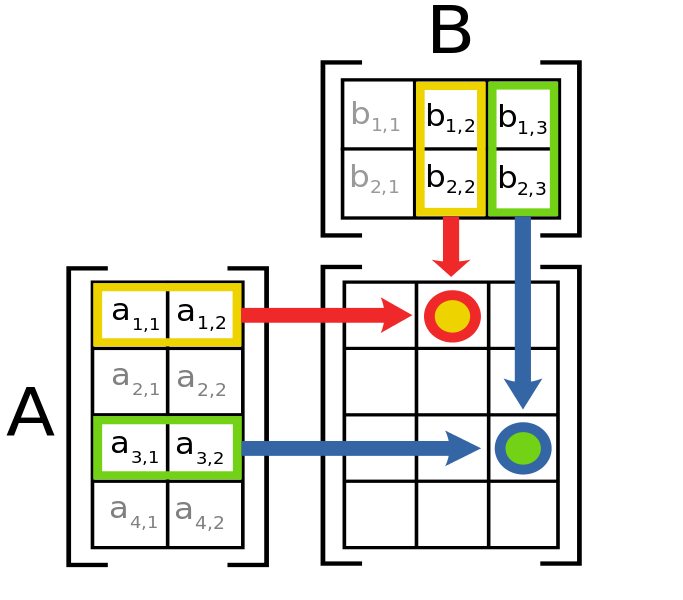
\includegraphics[width=0.7\linewidth]{matmul}
\caption{Matrix multiplication}
\end{figure}
If $\A\B = \C$, then we compute element $C_{ij}$ by taking the dot product of the $i$-th row of $\A$ and the $j$-th column of $\B$.

\noindent Note that the first matrix must have the same number of \emph{columns}, as the second has \emph{rows}. The other dimensions can be chosen freely.

One specific application of matrix multiplication is matrix-by-vector multiplication (where we see a column vector as just an $n$-by-$1$ matrix). The multiplication $\y = \W\x$ transforms vector $\x$ into vector $\y$. If $\W$ is a square matrix, this operation is a called a \emph{map}.

The notation $\x^T\y$ for the dot product should now be clear: we are matrix multiplying $\x$ (transposed to a row vector) by $\y$, resulting in a $1$-by-$1$ matrix.

Both the dot product and matrix multiplication have many different intuitive explanations. We don't have room to develop these intuitions here (follow the links below if you're curious), but throughout the course, you'll see different ways of using these concepts.

\qu Explain in words what the following notations represent:

\begin{enumerate}
\item $f: \R^3 \to \R^2$ \ans{$f$ is a function from the 3-dimensional Euclidean space to the 2-dimensional Euclidean space.}{}
\item $\y = \W \x$ \ans{The vector $\y$ is defined as the product of the matrix $\W$ and the vector $\x$}{}
\item $z = \y^T\x$ \ans{The scalar $z$ is defined as the the transposed vector $\y$ times the vector $\x$. This is also known as the \emph{dot product} of $\x$ and $\y$.}{}
\item $\W \in \R^{5 \times 4}$ \ans{$\W$ is a matrix with 5 rows, and 4 columns.}{}
\end{enumerate}

\indent In future, if you see unfamiliar notation, see if you can find the symbols in this page: \url{https://en.wikipedia.org/wiki/List_of_mathematical_symbols}. Even if that doesn't explain it fully, it may provide you with some keywords to google.

\qu Which of the following operations are possible, and which aren't?

\begin{enumerate}
\item Multiplying a $5 \times 4$ matrix by another $5 \times 4$ matrix. \ans{Impossible}{}
\item Element-wise multiplying a $5 \times 4$ matrix by another $5 \times 4$ matrix. \ans{Possible}{}
\item Multiplying a $5 \times 4$ matrix by a $4 \times 5$ matrix. \ans{Possible}{}
\item Multiplying a $5 \times 4$ matrix by a $4 \times 1$ matrix. \ans{Possible}{}
\item Element-wise multiplying a $5 \times 4$ matrix by a $4 \times 5$ matrix. \ans{Impossible}{}
\item Multiplying any matrix by its transpose. \ans{Always possible}{}
\item Element-wise multiplying any matrix by its transpose. \ans{Not always possible}{}
\item Element-wise multiplying a square matrix by its transpose. \ans{Always possible}{}
\end{enumerate}

\qu \noindent Which of the following is true?
	
\begin{enumerate}
\item Let $\U = \bc{\V}\oc{\W}$ for matrices $\U$, $\bc{\V}$, $\oc{\W}$. $U_{\rc{i}\gc{j}}$ is the dot product of the $\rc{i}$-th column of $\bc{\V}$ and the $\gc{j}$-th column of $\oc{\W}$. \ans{False}{}
\item Let $\U = \bc{\V}\oc{\W}$ for matrices $\U$, $\bc{\V}$, $\oc{\W}$. $U_{\rc{i}\gc{j}}$  is the dot product of the $\rc{i}$-th row of $\bc{\V}$ and the $\gc{j}$-th column of $\oc{\W}$. \ans{True}{}
\item Matrix multiplication is \emph{commutative}. \ans{False. It is not always true that $\V\W = \W\V$.}{}
\item Matrix multiplication is \emph{distributive}. \ans{True. Multiplication can always be \emph{distributed} over a sum: $\U(\V+\W) = \U\V + \U\W$ and $(\V+\W)\U = \V\U + \W\U$. Note that the order needs to be maintained: \rc{$\U(\V+\W) = \V\U + \W\U$} does \textbf{not} hold for all matrices.}{}

\item Matrix multiplication is \emph{associative}. \ans{True. Multiplying $\U$ by $\V$ and multiplying the result by $\W$ is the same as multiplying $\U$ by the result of multiplying $\V$ by $\W$: $(\U\V)\W) = \U(\V\W)$}{}
\item There exist matrices $\U$ and $\bc{\V}$ such that $\U\bc{\V} = \bc{\V}\U$. \ans{True. For instance, if one of them is the identity matrix, this always holds.}{}

\end{enumerate}


\qu
\begin{enumerate}
	\item The linear function $f(\pc{a}, \bc{b}, \rc{c}) = \alpha \pc{a} + \beta \bc{b} + \gamma \rc{c}$ can be written as the dot product of two vectors. What are the vectors? \ans{If $\x = (\pc{a}, \bc{b}, \rc{c})^T$ and $\bw = (\alpha, \beta, \gamma)^T$, then $f(x) = \bw^T\x$}{}
	\item The linear function $f(\pc{a}, \bc{b}, \rc{c}) = \alpha \pc{a} + \beta \bc{b} + \gamma \rc{c} + \delta$ can be also be written as the dot product of two vectors. What are the vectors? \ans{If $\x = (\pc{a}, \bc{b}, \rc{c}, 1)^T$ and $\bw = (\alpha, \beta, \gamma, \delta)^T$, then $f(x) = \bw^T\x$}{}
	\item The \emph{quadratic} function $f(\bc{a}, \oc{b}) = \alpha \bc{a}^2 + \beta \bc{a}\oc{b} + \gamma \oc{b}\bc{a} + \delta\oc{b}^2$ can be written as $f(\x) = \x^T\W\x$ (also known as a bilinear product). What should $\x$ and $\W$ be? \ans{$\x = \begin{bmatrix}\bc{a}\\ \oc{b}\end{bmatrix}$,$\W = \begin{bmatrix}\alpha & \beta \\ \gamma & \delta \end{bmatrix}$}{}
\end{enumerate}

\noindent If you found these exercises completely impossible, you should brush up on your Linear Algebra a little. You don't need much, the basics of vectors, matrices and matrix multiplication should do the trick. The following articles may help. If not, hunt around for one that explains things at your level:
\begin{itemize}
\item \url{https://betterexplained.com/articles/linear-algebra-guide/}
\item \url{https://www.khanacademy.org/math/linear-algebra}
\item \url{http://samples.jbpub.com/9781556229114/chapter7.pdf}
\end{itemize}
If you find anything that helps you, let us know on the discussion board.

\section{Calculus}

To denote the derivative of $f(\bc{x})$ we will use the notation $\frac{\kc{d}f(\bc{x})}{\kc{d}\bc{x}}$ (with $\kp$ taking the place of $\kc{d}$ for partial derivatives). You may be more comfortable with the notation $f'(\bc{x})$ for the derivative. I sympathize, but when it comes to machine learning, the former notation makes things \emph{much} simpler down the line, so I recommend getting used to it.

We will assume that you know the basics of calculus (specifically, taking 1D derivatives), so we won't offer an explanation here. Use the exercises below to check whether your understanding is sufficient. If not, practice using the links below.

\qu \noindent Let $f(\bc{x}) = 3\bc{x}^2 + 5\bc{x} + 1$ with $\bc{x}$ a scalar.
\begin{enumerate}
	\item What is the derivative of $f(\bc{x})$? \ans{$\frac{\kc{d}f(\bc{x})}{\kc{d}\bc{x}} = \frac{\kc{d} 3\bc{x}^2 + 5\bc{x} + 1}{\kc{d}\bc{x}} = \frac{\kc{d}3\bc{x}^2}{\kc{d}\bc{x}} + \frac{\kc{d}5\bc{x}}{\kc{d}\bc{x}} + \frac{\kc{d}1}{\kc{d}\bc{x}} = 3\frac{\kc{d}\bc{x}^2}{\kc{d}\bc{x}} + 5\frac{\kc{d}\bc{x}}{\kc{d}\bc{x}} + \frac{\kc{d}1}{\kc{d}\bc{x}} = 3\cdot2\bc{x} + 5\cdot1 + 0 = 6\bc{x} + 5$}{}
	\item For which $\bc{x}$ is $f(\bc{x})$ at its minimum? \ans{$\frac{\kc{d}f(\bc{x})}{\kc{d}\bc{x}} = 0$, $6\bc{x} + 5 = 0$, $\bc{x} = - \frac{5}{6}$}{}
	\item Let $h(\bc{x}) = g(f(\bc{x}))$, with $f$ defined as above. Let $\frac{\kc{d}g(\bc{x})}{\kc{d}\bc{x}} = \sin(\bc{x})/\bc{x}$. Without knowing what $g(\bc{x})$ is (or working it out), can we find the derivative of $h(\bc{x})$? \ans{Yes, using the \emph{chain rule}: \\$\frac{\kc{d}p(q(\bc{x}))}{\kc{d}\bc{x}} = \frac{\kc{d}p(q(\bc{x}))}{\kc{d}q(\bc{x})}\frac{\kc{d}q(\bc{x})}{\kc{d}\bc{x}}$. Thus $\frac{\kc{d}h(\bc{x})}{\kc{d}\bc{x}} = \frac{\kc{d}g(f(\bc{x}))}{\kc{d}\bc{x}} = \frac{\kc{d}g(f(\bc{x}))}{\kc{d}f(\bc{x})}\frac{\kc{d}f(\bc{x})}{\kc{d}\bc{x}} = \frac{\sin f(\bc{x})}{f(\bc{x})} (6x + 5) = \frac{\sin(3\bc{x}^2 + 5\bc{x} + 1)}{3\bc{x}^2 + 5x + 1}(6\bc{x} + 5)$.}{}
\end{enumerate}

\qu Let $\bc{\x} \in \R^2$ and let $f(\bc{\x}) = 3 {\bc{x_1}}^2 + 4 \bc{x_1}\bc{x_2} - {\bc{x_2}}^2$
\begin{enumerate}
\item What is the \emph{partial} derivative of $f(\bc{\x})$ with respect to $\bc{x_1}$? \ans{\[\frac{\kp\left ( 3 \bc{x_1}^2 + 4 \bc{x_1x_2} - \bc{x_2}^2\right ) }{\kp \bc{x_1}} = \frac{\kp 3\bc{x_1}^2}{\kp \bc{x_1}} + \frac{\kp 4 \bc{x_1x_2}}{\kp \bc{x_1}} - \frac{\kp \bc{x_2}^2}{\kp \bc{x_1}}  = 6\bc{x_1} + 4\bc{x_2} \]}{}
\item What is the partial derivative of $f(\bc{\x})$ with respect to $\bc{x_2}$? \ans{\[\frac{\kp 3\bc{x_1}^2}{\kp \bc{x_2}} + \frac{\kp 4 \bc{x_1x_2} }{\kp \bc{x_2}} - \frac{\kp \bc{x_2}^2}{\kp \bc{x_2}} = 4\bc{x_1} - 2\bc{x_2} \]}{}
\item What is the \emph{gradient} of $f(\bc{\x})$? \ans{The gradient is the vector of all partial derivatives: $\nabla f(\bc{\x}) = (6\bc{x_1} + 4\bc{x_2}, 4\bc{x_1} - 2 \bc{x_2})$. For practical reasons, the gradient is usually defined as a \emph{row} vector (when the input to $f$ is a column vector).}{}
\item The gradient is a function derived from $f$, just like the derivative is a function. What are the domain and range of the gradient of $f(\bc{\x})$?	 \ans{The gradient has the same input as $f$, so the domain is also $\R^2$. The gradient defines a vector of length two for each input, so its range is $\R^2$. In other words $\nabla f: \R^2 \to \R^2$.}{}
\end{enumerate}

\noindent As before, if you found these exercises tricky, even after reading the answers, you should probably brush up a little on your calculus. Here are some links you may find helpful.
\begin{itemize}
\item \url{https://betterexplained.com/articles/vector-calculus-understanding-the-gradient/}
\item \url{https://www.khanacademy.org/math/multivariable-calculus/multivariable-derivatives/partial-derivative-and-gradient-articles/a/introduction-to-partial-derivatives}
\item \url{http://tutorial.math.lamar.edu/Classes/CalcIII/PartialDerivatives.aspx}
\end{itemize}


\end{document}
